\section{Methods}
\subsection{Dataset}
The dataset is data collected from the Children’s Hospital Boston, consisting in EEG recordings of subjects with intractable seizures. The folders classify in 23 cases from 22 subjects (case chb21 and chb1 are the same but 1.5 years apart). The subject’s personal information gender and age is in a separate file called SUBJECT-INFO added in this paper as subject\_info.csv.
\\\\
Each case contains between 9 and 42 edf files. There are edf files of EEG signals without seizures and others with recordings of seizures, these defined in RECORDS-WITH-SEIZURES. The files with seizures have the extension edf.seizures which disables the possibility of accessing the file with a normal edf reader library. The seizure data can be read from the summary file.
\\
\begin{figure}[h!]
  \caption{The international 10-20 system defining electrodes position seen from different views}
  \centering
  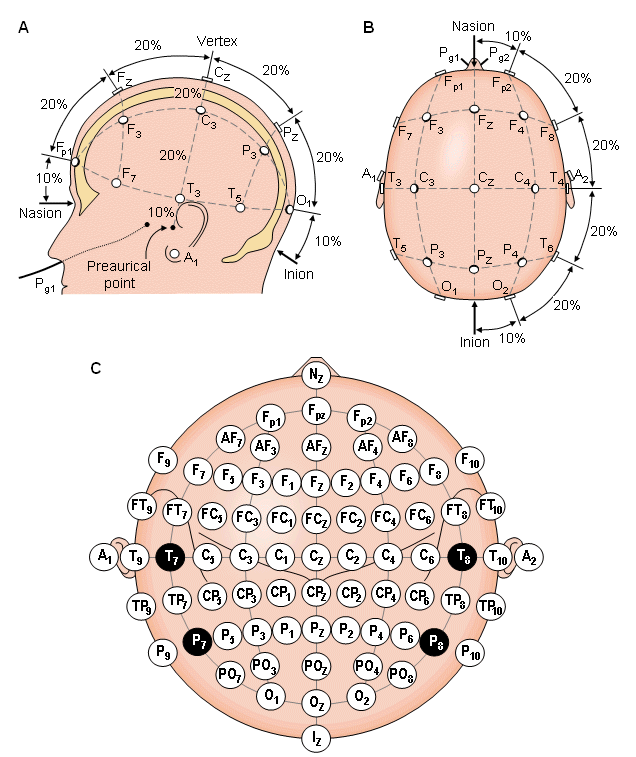
\includegraphics[width=0.5\textwidth]{img/electrodesposiiton.png}
\end{figure}
\\
Most cases have 1 hour of EEG recordings, but some have 1 to 4 hours depending on the case, split between 9 to 42 edf recordings, recorded at 256Hz in 16 bit resolution. The position of the electrodes as well as the nomenclature are in the International 10-20 system.
\\\\
It’s important to note, some subjects had hardware interruptions while the recording of the EEG, and so when there is an interruption, it’s noted in the summary.txt file. This kind of interruptions are a problem to get information normally, because the disposition of the electrodes change making it harder to control the disposition of the electrodes and the EEG might not work for a sequential approach, for example, if it’s important there is hypothetically an order on how a seizure comes to be, this file would certainly be discarded. To take into account this file the script to process the data in this TFG should be programmed to do so. For now, the objective is different, this project just classifies if there is or not a seizure, but for further development it should be considered. The data base is very large containing enough uninterrupted data to work with.
\\\\
The data used to train the model in this TFG is data from subject 1 to subject 10. Also, only few edf in each subject’s folders have any seizure. If every edf was used, there would be a lot more data labelled as not seizure than seizure data, so from each subject only the files with seizures are used. Even so, handling only files with seizures the dataset is still unbalanced, so for future development two strategies should be considered:
\\
\begin{itemize}
  \item Files should be cut to have a balance of labelled data of 50\% data with seizure and 50\% data without. This strategy could end up in subsampling, considering there are few seizures in the hole dataset.
  \item When training the model, the criteria of cross Entropy should be weighted. To consider no seizure less important than seizure data.
\end{itemize}
\leavevmode\\
\subsection{Data processing}
Because in this TFG the CHB-MIT Scalp EEG Database is being used and all files are in format edf, a first script has been needed to process data, called “03\_ReadEDF.py”.
\\\\
In the “03\_ReadEDF.py” script there are different options on how raw data is imported, and also there are options on the way to execute them. During the development of this TFG many tests have been done, there for there are two different ways to execute the script:
\\
\begin{itemize}
  \item Single execution, where the subject number and the edf file of the subject needs to be provided to execute the script for this single file. 
  \item Multiple executions, where the number of subjects is provided. The script will go through all the first n subjects defined.
\end{itemize}
\leavevmode\\
It’s designed to extract the files from a specific folder hierarchy where all the encephalograms are classified by subjects. For simplicity this script obtains, filters, plots, and saves in parquets all input data. Afterword’s it also labels the data and splits it into windows so the model can process data easily. 
\\\\
The script will automatically label all raw data using the summary file in each subject’s folder, so it’s important for it to be present or a label execution error will pop up. The files edf.seizures in every subject’s folder were unreadable, even reading the binary was a failure. The script will make sure the file has all the data from the desired electrodes, this is important because there were hardware problems while recording the edfs, some files have gaps or lack some data, if any edf file has this problem it will automatically be excluded and the user will be notified. Each one has 22 different channels, which are the electrodes of the subject. In order to label the data, a new column is created (the 23rd) as seizure with the information of every row being a seizure or not and also a 24th column to set the observation windows for the model.
\\\\
Filtering data is done by first setting a maximum range from 0.5hz to 50hz, and afterwards only by changing the name of a parameter it can be changed to delta, theta, alpha, beta or gamma’s range frequencies in a dictionary added by default. Everything is modular so it can be changed any time with any range of frequencies. All data is saved in parquet format in a different folder, if plotting is enabled it will plot each subject’s data.
\\\\
Once the data is filtered and labelled it`s saved two numpys, one “file\_data\_x.npy” and “file\_data\_y.npy”. In data\_x the file has a numpy array of three dimensions containing number of windows, electrodes and values. In data\_y there are two dimensions, number of windows and window\_seizure which defines if the window has a seizure in it with a 1 or not with a 0. 
\\\\
With this, all the parquets and arrays are specifically saved and ordered to ensure easy access and fast comprehension of the hierarchy of folders. The database folder has every subject in a separate folder and inside individual folders for edf, parquets, numpys and results.
\\
\begin{figure}[h!]
    \caption{Filtered data in Theta range from electrode FP1-F7, subject 1 file 3}
    \centering
    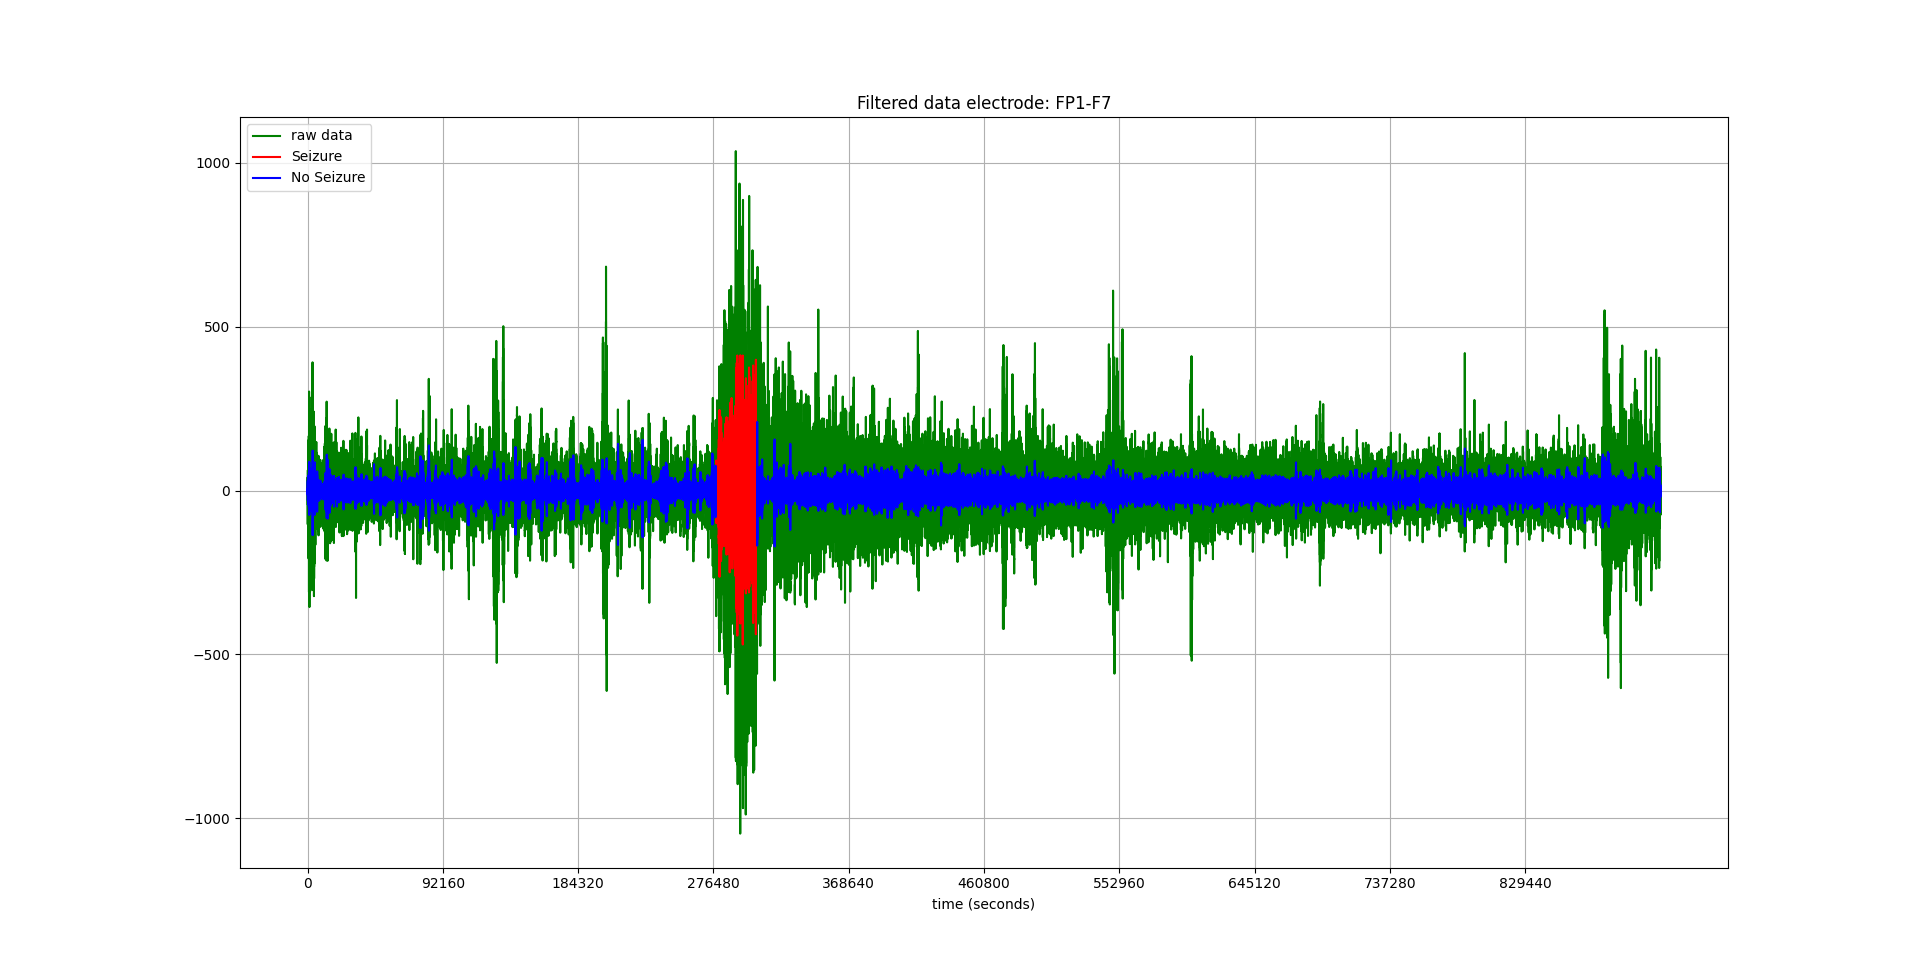
\includegraphics[width=0.5\textwidth]{img/all in one.png}
\end{figure}

\leavevmode\\
\subsection{Network}
An already done deep learning algorithm is used from the research group IAM from the CVC, which is working on a framework to determine the optimal architecture for cognitive state recognition from EEG signals, with the objective to answer different questions:
\\
\begin{itemize}
  \item How to combine the signals to create the input features for feature extraction? In this case, having 14 sensors x 5 wavelengths, so 70 raw signals. These signals can be concatenated, or projected.
  \item Which neural network is the best performer?
  \item Is it better to ensemble the different classifiers before combining the signals?
\end{itemize}
\leavevmode\\
This model was originally intended to study brain workload, so, with the help of this model it’s changed to fulfil the objective of clinic seizure detection. In this TFG, different strategies are applied on the input data of the algorithm to further study it’s capabilities as well as using different models to compare results between them.
\\\\
Once all desired raw data is filtered and saved, the second script to execute is “04\_MExecution.py”, this one is in charge of the execution of the model, training and testing to obtain the results classifying the data. All hyperparameters are defined at the beginning of the script as well as the declaration and initialization of the model. There are different typs of execution for development that can be enabled by boolean variables commented in the script. 
\\
\begin{itemize}
  \item CheckModel is the first way to execute the model, this one is needed to make sure the model works as intended before using real data to train it. It uses the selected model and feeds to it random data using torch with the defined parameters in the function.
  \item If the model works with no isues with CheckModel, then the training execution can begin. This first phase selects every numpy from n subjects defined at the beginning and trains the model with all the data. Every time the model finishes the epochs of a file, it saves the model in the database.
  \item In the second phase the previous trained model is loaded to test it and data is defined to set the normalization scalers for testing. For further development this should be changed to make an average of scalers by all trained data for example, or normalize data before the script’s execution. Once the model is tested a classification report is done using sklearn library and saved to a results folder in the subject’s folder.
\end{itemize}
\leavevmode\\
\\
The script uses numpy arrays as input data stored as previously mentioned in data\_x and data\_y. These files depending on the strategy of the script can be processed one last time to ensure good results from the classification. In this TFG data when loaded uses the strategy stated previously as phase 1 and 2, for training and testing. But the script has the option to split the files in train and test by a percentage variable. For the executions done this variable is set to 1 (100\%) on training, and 0 on testing phase to consider all the data from the file for the purpose of training or testing.
\\\\
During the implementation of this script, a lot of problems of dependency on critical libraries has happened. Starting by cuda, for faster results it is used in all models, but it might not work if the architecture of the graphics card is too old. It is also not compatible with python 3.10 which was the version being worked on at the moment, it had to be switched to an environment with python 3.8 to avoid further issues. The script will be executed with cuda if the libraries are available as well as the drivers, if not it will automatically work with the CPU.
\\\\
When it’s time to save the model, it’s saved in a folder called “trys” in the root directory, like if it was another subject but it only contains pt files. The name of the file is automatically created defined by the last subject and file executed, as well as the date considering day, month, year, hour, minute and second when the file got saved. Seconds where necessary to save in the name as well to prevent models from overwriting if it had to be saved in the same minute because of low epoch training.
\\\\
The models used in the TFG have similar structures. The first one CNN\_ConcatInput and the second one CNN\_ProjOut\_Conv. As the names suggest these models are Convolutional Neural Networks. Both models have 3 base layers of convolution defined by a function ConVNet which defines 3 different layers using torch, the first one being 16@22x19. The first parameter as number of input features defined by a constant variable defined in the constructor of the model, the second parameter defines the size of the data, 22 being the channels, in this case 
\\
\leavevmode\\
\begin{figure}[h!]
  \caption{Scheme of data dimension transformation through model CNN\_ConcatInput}
  \centering
  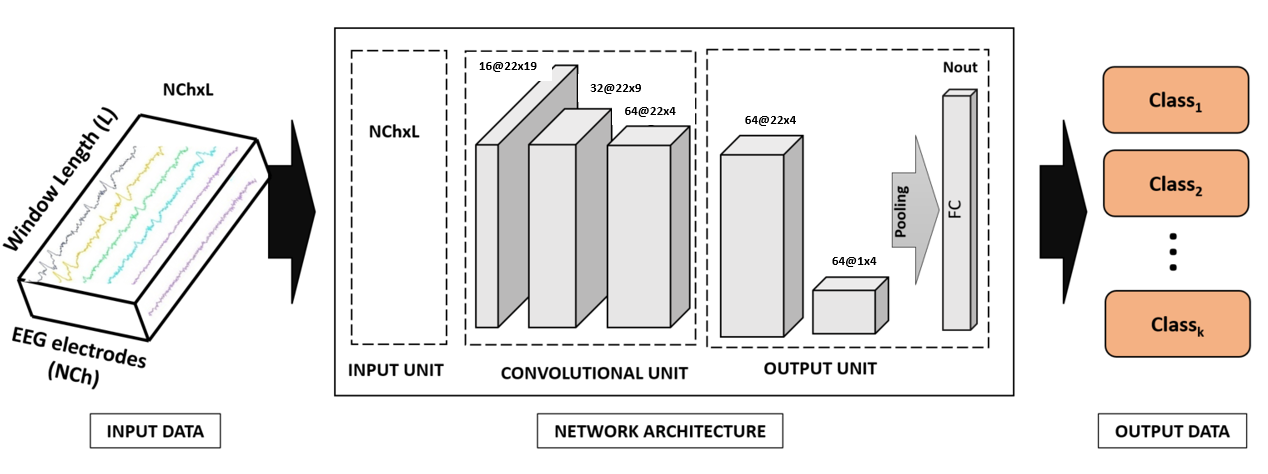
\includegraphics[width=0.5\textwidth]{img/FeatureProjectorModel CHM.png}
\end{figure}
\leavevmode\\
During the implementation of this procedure, a lot of problems of dependency on critical libraries has happened. Starting by cuda, for faster results it is used in all models, but it might not work if the architecture of the graphics card is too old. It is also not compatible with python 3.10 which was the version being worked on at the moment, it had to be switched to an environment with python 3.8 to avoid further issues.
\\

